\task{Катим круг}
\noindent В «нижней» точке $P$ окружности радиуса $R$ её касается круг радиуса $\tfrac{R}{2}$, «нижняя» точка которого, в свою очередь, отмечена (см.\,рисунок). Круг начинают «вкатывать» вверх по окружности так, что в точке соприкосновения они никогда не скользят друг относительно друга.

\centerline{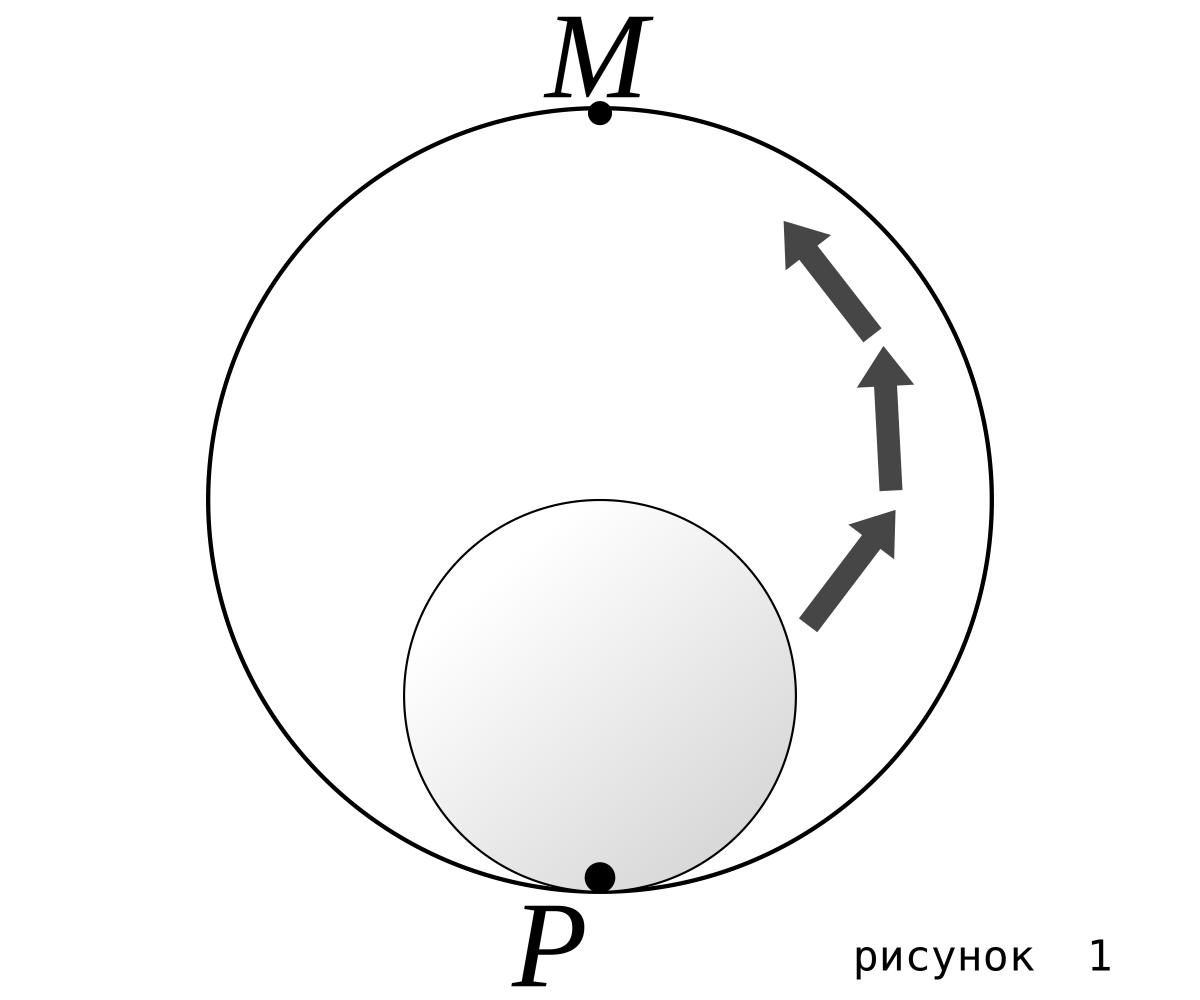
\includegraphics[width=5.5cm]{stats/2018/images/circle-move}}

\begin{enumerate}
\itA Докажите, что когда круг проедет пол-оборота по окружности и будет касаться её в точке $M$, то его отмеченная точка окажется там же, в точке $M$.

\itB Докажите, что в любой момент времени точка касания круга с ок-\linebreak ружностью и отмеченная точка круга находятся на одной горизонтальной прямой.

\itC Докажите, что отмеченная точка перемещается строго по вертикальному отрезку.
\end{enumerate}